\chapter{Protótipo}
\label{AppendixC}
Neste apêndice são mostrados alguns artefactos recolhidos ao longo das fases de conceção, desenvolvimento e validação do protótipo.

\section{Configuração}
Nesta secção apresentam-se algumas imagens referentes ao processo de configuração levado no protótipo.
%
\begin{figure}[!ht]
    \centering
    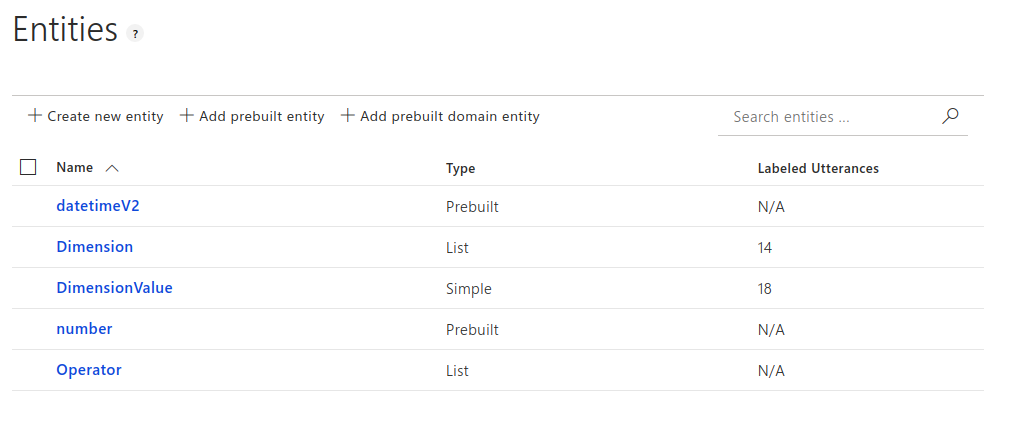
\includegraphics[width=\textwidth]{appendices/assets/kb07.png}
    \caption{Definição das entidades esperadas}
\end{figure}
%
\begin{figure}
\centering
    \begin{subfigure}{.9\textwidth}
        \centering
        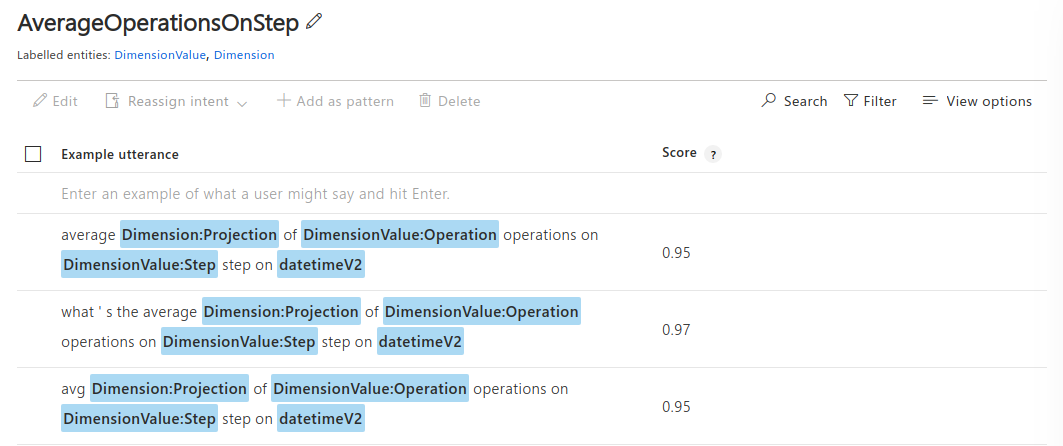
\includegraphics[width=\textwidth]{appendices/assets/kb01.png}
        \caption{Intenção \textit{AverageOperationOnStep}}
     \end{subfigure}
     \begin{subfigure}{.9\textwidth}
         \centering
        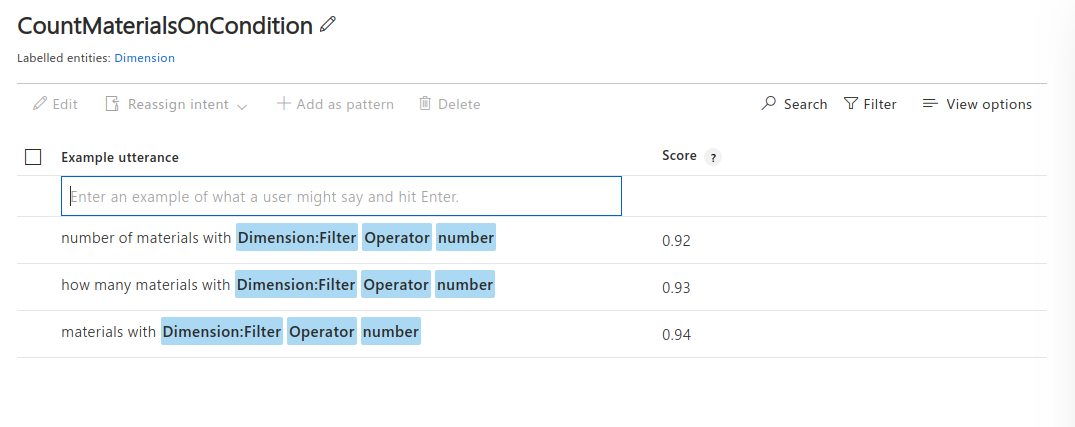
\includegraphics[width=\textwidth]{appendices/assets/kb02.png}
        \caption{Intenção \textit{CountMaterialsOnCondition}}
     \end{subfigure}
     \begin{subfigure}{.9\textwidth}
        \centering
        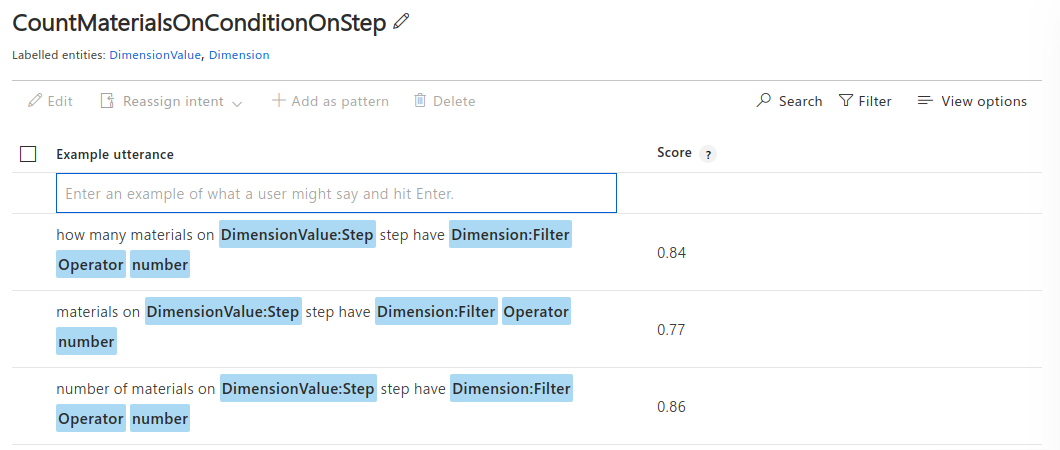
\includegraphics[width=\textwidth]{appendices/assets/kb03.png}
        \caption{Intenção \textit{CountMaterialsOnConditionOnStep}}
     \end{subfigure}
\caption{Intenções definidas, contendo as expressões e respetivas entidades}
\end{figure}
%
\begin{figure}
    \centering
         \begin{subfigure}{.9\textwidth}
        \centering
        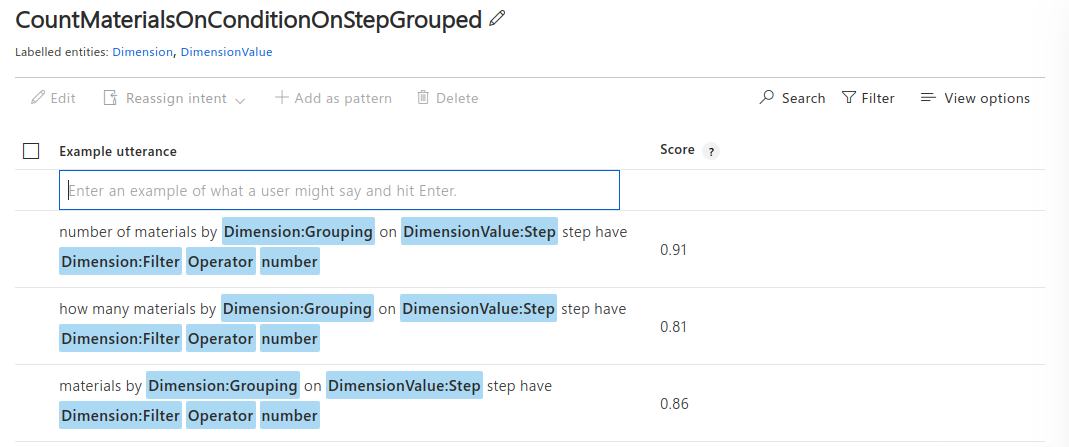
\includegraphics[width=\textwidth]{appendices/assets/kb04.png}
        \caption{Intenção \textit{CountMaterialsOnConditionOnStepGrouped}}
     \end{subfigure}
     \begin{subfigure}{.9\textwidth}
        \centering
        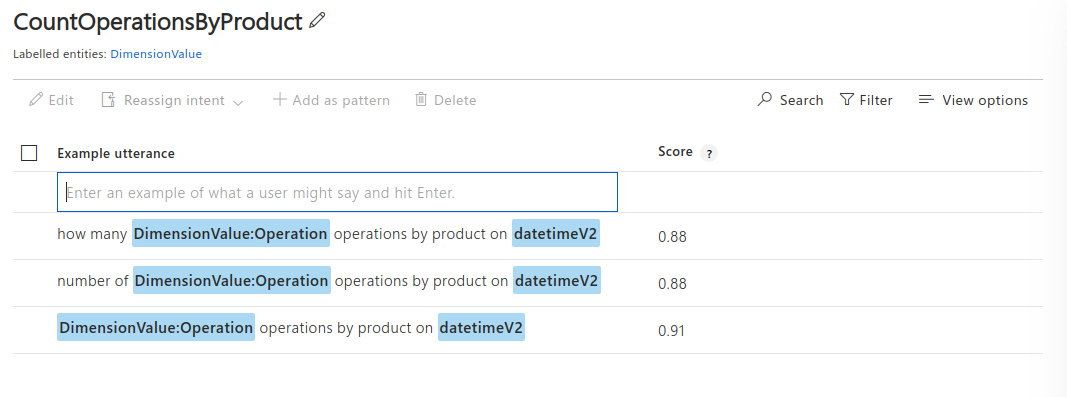
\includegraphics[width=\textwidth]{appendices/assets/kb05.png}
        \caption{Intenção \textit{CountOperationsByProduct}}
     \end{subfigure}
     \begin{subfigure}{.9\textwidth}
        \centering
        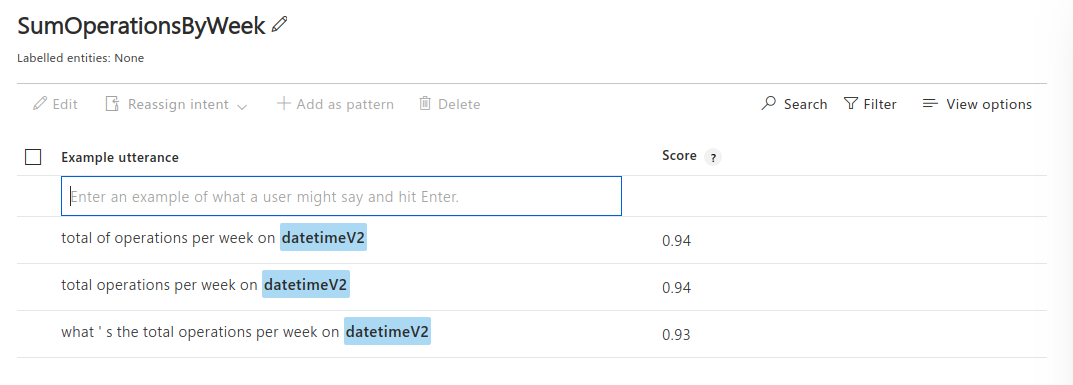
\includegraphics[width=\textwidth]{appendices/assets/kb06.png}
        \caption{Intenção \textit{SumOperationsByWeek}}
     \end{subfigure}
    \caption{Continuação das intenções definidas, contendo as expressões e respetivas entidades}
\end{figure}

\clearpage

\section{Validação}
Nesta secção apresentam-se algumas imagens referentes ao processo de validação do protótipo.

\begin{figure}[!ht]
\centering
    \begin{subfigure}{.48\textwidth}
        \centering
        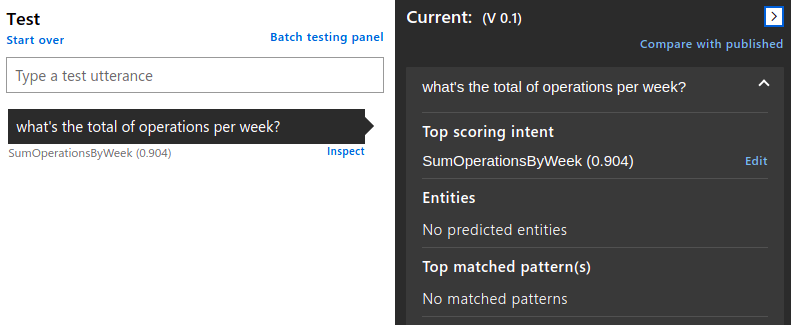
\includegraphics[width=\textwidth]{appendices/assets/nlcomprehension01.png}
        \caption{Intenção \textit{SumOperationsByWeek}}
     \end{subfigure}
     \begin{subfigure}{.48\textwidth}
         \centering
        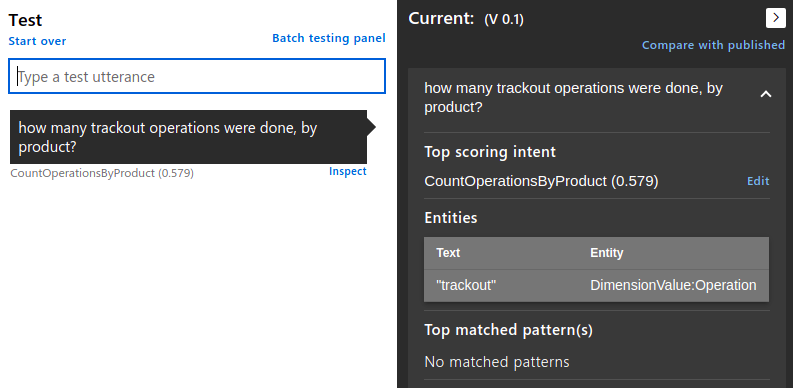
\includegraphics[width=\textwidth]{appendices/assets/nlcomprehension02.png}
        \caption{Intenção \textit{CountOperationByProduct}}
     \end{subfigure}
     \bigbreak
     \begin{subfigure}{.48\textwidth}
        \centering
        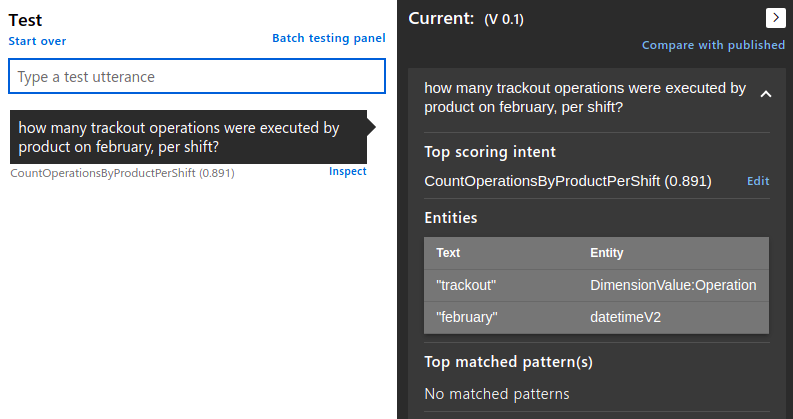
\includegraphics[width=\textwidth]{appendices/assets/nlcomprehension03.png}
        \caption{Intenção \textit{AverageOperationsOnStep}}
     \end{subfigure}
     \begin{subfigure}{.48\textwidth}
        \centering
        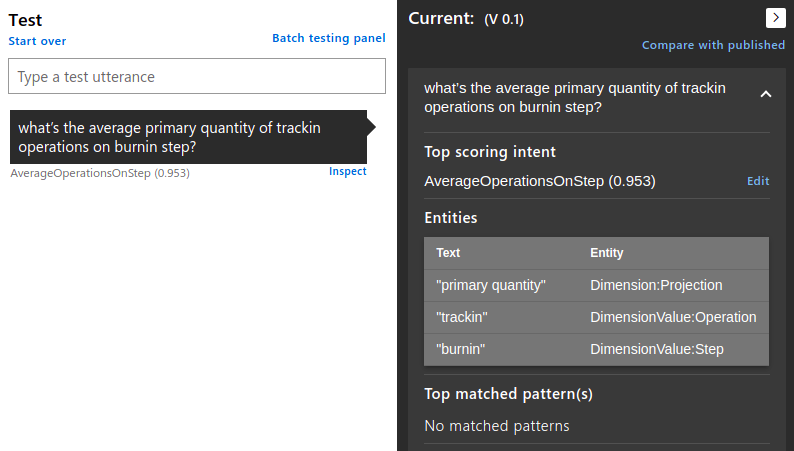
\includegraphics[width=\textwidth]{appendices/assets/nlcomprehension04.png}
        \caption{Intenção \textit{CountOperationsOnConditionOnStepGrouped}}
     \end{subfigure}
     \bigbreak
     \begin{subfigure}{.48\textwidth}
        \centering
        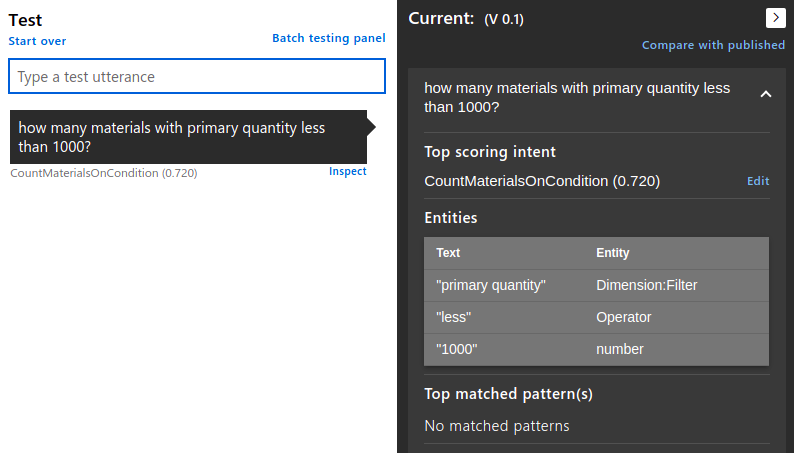
\includegraphics[width=\textwidth]{appendices/assets/nlcomprehension05.png}
        \caption{Intenção \textit{AverageOperationsOnStep}}
     \end{subfigure}
     \begin{subfigure}{.48\textwidth}
        \centering
        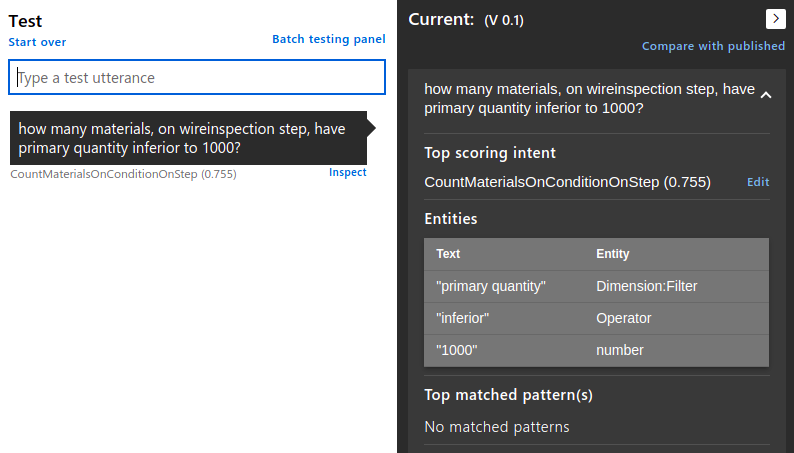
\includegraphics[width=\textwidth]{appendices/assets/nlcomprehension06.png}
        \caption{Intenção \textit{CountOperationsOnConditionOnStepGrouped}}
     \end{subfigure}
\caption{Outras imagens relativas à avaliação de intenções e entidades do protótipo}
\label{fig:nlcomprehesion_others}
\end{figure}